% !TeX encoding = UTF-8

\chapter{TESTES E ANÁLISE DOS RESULTADOS}\label{ch:resultados}

Este capítulo tem como finalidade apresentar os testes realizados através da manipulação das constantes definidas na \autoref{sec:consts}, seus resultados e posteriormente, a análise dos mesmos.

\section{Ambiente de Testes}\label{sec:ambtest}

Os testes foram realizados no local de trabalho do autor e os objetos de testes foram as faces dos funcionários do escritório do mesmo, dentro os quais a participação variava diariamente entre 6 a 10 participantes, incluindo o autor. Tomou-se cuidado para que as faces relacionadas fossem sempre as mesmas. Ou seja, a "face 1"\ seria a mesma face em todos os dias de treino.

Os equipamentos (\textit{hardwares}), descritos na \autoref{sub-hardw}, foram postos em um local de saída dos funcionários do escritóio, onde as condições luminosas eram sempre as mesmas.

A interface do sistema, como se pode ver na \autoref{screenshot-sys}, dispõe de uma máscara que indica o local em que a face deve ser posicionada corretamente em frente a câmera, e a câmera posicionada no mesmo local em todos os testes. A cada dia, caso o resultado de correspondência fosse considerada ruim (muito acima do valor mínimo \textit{MIN\_DIST}), ou caso o objeto de teste tenha se movido no momento do treino interrompendo o processo, a face poderia ser treinada novamente, o que acumularia as faces de treino do objeto de teste.

\begin{figure}[h]
	\centering
	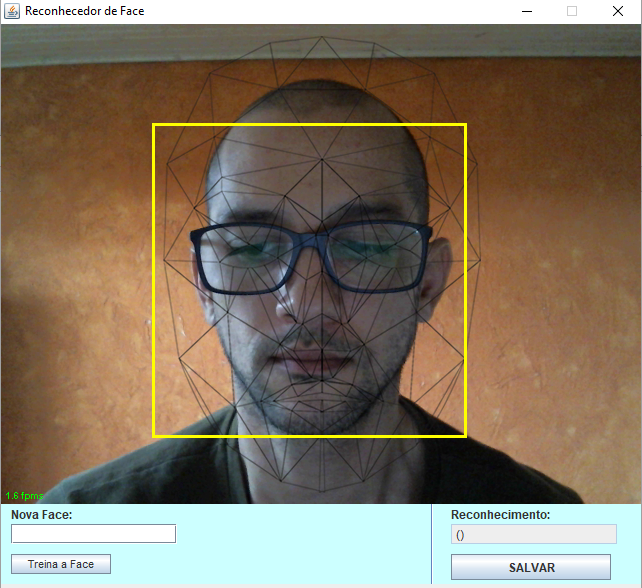
\includegraphics[width=1\textwidth]{screenshot-sys}
	\caption{Imagem do Sistema em Funcionamento.}
	\fonte{Elaborado pelo autor.}
	\label{screenshot-sys}
\end{figure}

Os usuários foram sujeitos ao teste sempre na mesma ordem. As faces dos objetos de testes foram expostas durante o tempo necessário para o sistema coletar a quantidade estabelecida pela constante \textit{NUM\_FACES\_TREINO}. O sistema foi configurado para faser cerca de 3 a 4 deteções por segundo.

Os testes documentados foram realizados em 5 (cinco) dias e divididos em três fases: duas fases de dois e uma fase de um dias. Para cada fase uma configuração distinta das constantes de controle contempladas na \autoref{sec:consts} foram definidas, as quais são detalhadas na seção seguinte.

Apresentam-se os resultados dos testes do sistema nas condições de cada fase em tabelas: uma para cada dia de teste. Todas apresentam as contagens das quantidades de reconhecimento realizadas por pessoa, bem como a nota média das distâncias correspodentes aos resultados de cada reconhecimento, tanto na falha quanto no sucesso, e a contagem de falsos positivos e falsos negativos.

A contagem dos resultados falsos positivos e falsos negativos foram feitos a olho nú e devidamente registrados pelo analista, comparando os resultados registrados pelo sistema no momento dos testes, como descreve a \autoref{sec:defsucregoc}.

\section{Testes e Resultados}\label{ch:testresult}

Esta sessão de testes, foi dividida em três fases: uma para cada configuração das constantes de controle. A finalidade de cada constante é contemplada na \autoref{sec:consts} e suas interações com o código descritas durante \autoref{sec:codigo}.


\subsection{Fase 1}\label{ch:testresultfaz1}
Para a primeira fase da \textit{sprint} testes, feita em dois dias, os valores das constantes de controle foram configuradas como define a lista abaixo.

\begin{itemize}	
	\item \textbf{NUM\_FACES\_TREINO = 2}
	\begin{itemize}	
		\item esta constante é resposável por controlar o número de faces a ser usado no treinamento, foi configurado para o valor 2 (dois) esperando-se manter um número reduzido de faces para treinamento, e consequentemente do tamanho do espaço multidimensional a ser gerado;
	\end{itemize}

	\item \textbf{NUM\_EF\_recog = 5}
	\begin{itemize}	
		\item esta constante é resposável por controlar o número de \textit{eigenfaces} ou auto-vetores a serem usadas no reconhecimento, foi configurado para o valor 5 (cinco), para se observar os resultados iniciais do experimento;
	\end{itemize}

	\item \textbf{MIN\_DIST = 0.433}
	\begin{itemize}	
		\item esta constante define se a distância encontrada na fase de reconhecimento pode ser considerada um resultado de sucesso ou falha, foi definida para o valor 0.433, para se observer os resultados iniciais.
	\end{itemize}
\end{itemize}

Estes valores iniciais foram definidos pelo desenvolvedor a partir de testes unitários não documentados em \textit{sprints} anteriores durante o desenvolvimento do sistema, onde os objetos de teste eram a face do próprio desenvolvedor, voluntários esporádicos ou imagens de faces.

Os resultados do primeiro dia de teste desta fase é descrito na \autoref{tab-res-fase1dia1}. Neste dia houveram 18 imagens de treinamento coletadas, com destaque para a "face 5", que por alguma razão, talvez sua pele muito branca e oleosa, refletia as luzes do ambiente dificultando o processo e apresentando maus resultados, e assim foi efetuada a coleta de mais imagens de treino deste usuário.

\begin{table}[h]
	\centering
	\caption{Resultado dos testes (Fase 1 - Primeiro dia) }
	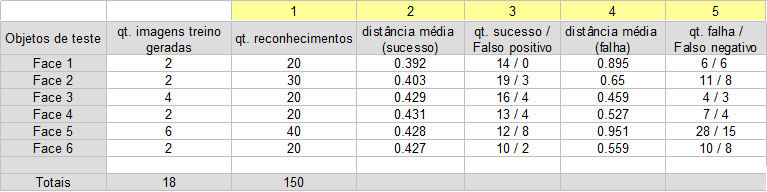
\includegraphics[width=1\textwidth]{tab-res-fase1dia1}
	\fonte{Elaborado pelo autor.}
	\label{tab-res-fase1dia1}
\end{table}

Os resultados do segundo dia de teste são apresentados na \autoref{tab-res-fase1dia2}. O esperado era que os usuários fossem reconhecidos com resultados parecidos. Observa-se que a "face 2 e 3"\ obtiveram maus resultados e tiveram que ser treinadas, possivelmente por faserem uso de maquiagem. A "face 5"\ continuou obtendo os maus resultados de anteriormente. Mais 4 faces foram adicionadas, acumulando um total de 22 imagens usadas para o treinamento.

\begin{table}[h]
	\centering
	\caption{Resultado dos testes (Fase 1 - Segundo dia) }
	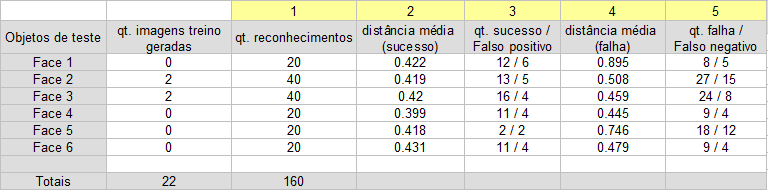
\includegraphics[width=1\textwidth]{tab-res-fase1dia2}
	\fonte{Elaborado pelo autor.}
	\label{tab-res-fase1dia2}
\end{table}



\subsection{Fase 2}\label{ch:testresultfaz2}
Para a segunda fase da \textit{sprint} testes, feita em dois dias, os valores das constantes de controle foram configuradas como define a lista abaixo. 

\begin{itemize}	
	\item \textbf{NUM\_FACES\_TREINO = 1}
	\begin{itemize}	
		\item esta constante é resposável por controlar o número de faces a ser usado no treinamento, foi configurado para o valor 1 (um) esperando-se reduzir ainda mais o espeço (em 50\%) para observar se diminui o numero de falsos positivos;
	\end{itemize}
	
	\item \textbf{NUM\_EF\_recog = 2}
	\begin{itemize}	
		\item esta constante foi configurado para o valor 2 (dois), para priozirar as \textit{eigenfaces} com mais probabilidade de ter atributos distintos entre as faces de treinamento, esperando-se observar um numero menor de falsos positivos
	\end{itemize}
	
	\item \textbf{MIN\_DIST = 0.55}
	\begin{itemize}	
		\item esta constante foi definida para o valor "0.55", esperando-se obervar uma melhor taxa de sucesso no reconhecimento.
	\end{itemize}
\end{itemize}

Os resultados do primeiro dia de teste desta fase é descrito na \autoref{tab-res-fase2dia1}. Neste dia coletou-se imagens de treino apenas de novos usuários, acumulando um total de 28 imagens de treino. 


\begin{table}[h]
	\centering
	\caption{Resultado dos testes (Fase 2 - Primeiro dia) }
	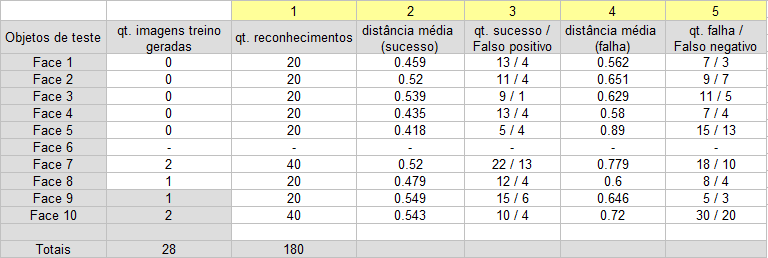
\includegraphics[width=1\textwidth]{tab-res-fase2dia1}
	\fonte{Elaborado pelo autor.}
	\label{tab-res-fase2dia1}
\end{table}


Os resultados do segundo dia de teste desta fase é descrito na \autoref{tab-res-fase2dia2}. Neste dia coletou-se uma imagem de cada usuário, acumulando um total de 35 imagens de treino. Foram feitos mais iterações de reconhecimento no usuário "face 5"\ pois este continuara a apresentar resultados maus (valores muito altos).


\begin{table}[h]
	\centering
	\caption{Resultado dos testes (Fase 2 - Segundo dia) }
	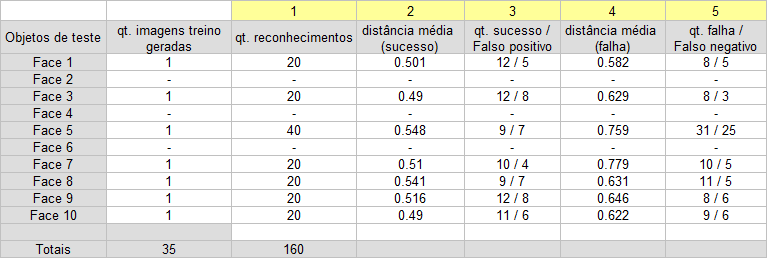
\includegraphics[width=1\textwidth]{tab-res-fase2dia2}
	\fonte{Elaborado pelo autor.}
	\label{tab-res-fase2dia2}
\end{table}



\subsection{Fase 3}\label{ch:testresultfaz3}
Para a terceira e últimas fase com apenas uma oportunidade para teste, as faces de treino foram deletadas para que se comece o teste com o espaço \textit{eigenspace} limpo/ Os valores das constantes de controle foram configuradas como define a lista abaixo.

\begin{itemize}	
	\item \textbf{NUM\_FACES\_TREINO = 7}
	\begin{itemize}	
		\item esta constante é resposável por controlar o número de faces a ser usado no treinamento, foi configurado para o valor 7 (sete) nesta fase, obter um valor maior de \textit{eigenfaces} geradas;
	\end{itemize}
	
	\item \textbf{NUM\_EF\_recog = 1}
	\begin{itemize}	
		\item esta constante foi configurado para o valor 1 (um), para descartar o máximo de \textit{eigenfaces} possível, afim de diminuir o número de falsos positivos;
	\end{itemize}
	
	\item \textbf{MIN\_DIST = 0.69}
	\begin{itemize}	
		\item esta constante foi definida para o valor "0.69", pois ao observar o teste anterior, analisou-se que em geral os resultados estavam piorando a medida que o número de imagens de treno aumentavam, e em muitos casos haviam muitos falsos negativos que poderiam ser confimação de sucesso.
	\end{itemize}
\end{itemize}

Os resultados desta fase de teste são apresentos na \autoref{tab-res-fase3}. Neste dia coletou-se 14 imagens de cada usuário, acumulando um total de 98 imagens de treino. Foram feitos mais iterações de reconhecimento para se ter uma melhor amostragem.

\begin{table}[h]
	\centering
	\caption{Resultado dos testes (Fase 3) }
	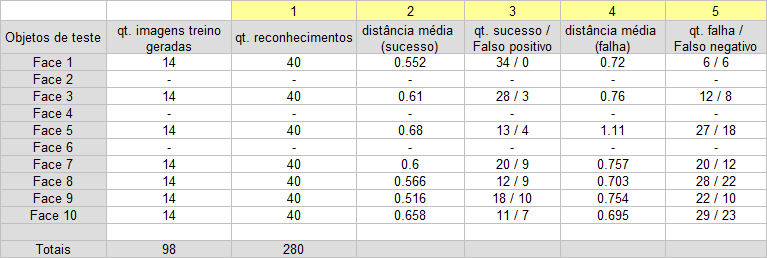
\includegraphics[width=1\textwidth]{tab-res-fase3}
	\fonte{Elaborado pelo autor.}
	\label{tab-res-fase3}
\end{table}





\section{Análise dos Resultados}\label{ch:analresult}

Ao decorrer dos testes e se analisar os resultados iniciais, pode-se perceber logo de início que a técnica é extremamente sensível a luzes/sombras, poses e expressões. Algo que pode variar muito a reflexão da luz na face do usuário é a cor da pele, oleosidade, maquiagem e acessórios como boné ou chapéu. Um mínimo movimento no momento da coleta das imagens de treino pode causar uma grande diferença no resultado.

Como se pode verificar na \autoref{taxarecogfases}, na primeira fase foram feitos 310 reconhecimentos sendo que 149 foram considerados pelo sistema como sucesso. Destes, apenas 103 foram de fato equivalentes, apresentando a taxa real de reconhecimento com \textit{33.22\%} de sucesso. Dos reconhecimentos considerados como falha somaram o total de 161, dos quais 92 eram falsos negativos, pois se tratava de uma real equivalência. Sendo assim, 55\% das falhas deveriam ser reconhecimento de sucesso. 

\begin{table}[h]
	\centering
	\caption{Taxas de sucesso reais dos reconhecimentos nas fases de teste.}
	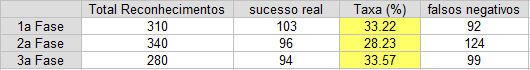
\includegraphics[width=.8\textwidth]{taxarecogfases}
	\fonte{Elaborado pelo autor.}
	\label{taxarecogfases}
\end{table}

Observou-se, que dependendo da face e suas condições, as médias das distâncias euclidianas poderiam variar forma imprevisível. Algumas faces tinham bons resultados de reconhecimento enquanto outras os apresentavam péssimos, em relação à constante \textit{MIN\_DIST}. O grande número de falsos negativos apresentados incentivaram a reconfiguração da constante \textit{MIN\_DIST} para um valor maior, \textit{NUM\_FACES\_TREINO} foi reduzido para que o espaço não sofresse muita adição de tamanho, \textit{NUM\_EF} foi reduzido para priorizar \textit{eigenfaces}, e apenas treinos de novas faces foram realizadas, esperando-se que os resultados de reconhecimento melhorassem ou se mantivessem.


Na segunda fase foram feitos 340 reconhecimentos sendo que 185 foram considerados pelo sistema como sucesso. Destes, 96 foram de fato equivalentes. Sendo assim, apresentando a taxa real de reconhecimento de \textit{28.3\%} de sucesso. Dos reconhecimentos considerados como falha, que somaram o total de 195, 124 se tratavam de uma real equivalência. Sendo assim 63.5\% das falhas deveriam ser reconhecimento de sucesso.

Observa-se que,os resultados da segunda fase foram piores que o da anterior, porém as contagens de falsos positivos e negativos ainda se apresentavam elevadas. Reconfigurou-se então as variáveis como conta na \autoref{ch:testresultfaz3} levando em conta lógica de que se um maior número de possível da coleta de imagens de uma face para o treino, combinado com o descarte de auto-vetores por auto-valores, "filtraria"\ melhor as caracteristicas da face e suas variáveis (sombras e reflexoes, movimentos, feiçoes ou enquadramento da face) melhor registradas. A constante \textit{MIN\_DIST} também sofreu adição de valores para que se diminuíse ainda mais os falsos negativos que poderiam ser reconhecimentos de sucesso, com cautela para não provocar resultados falsos positivos.

Segundo os resultados da terceira fase, foram feitos 280 reconhecimentos sendo que 136 foram considerados pelo sistema como sucesso. Destes, apenas 94 foram de fato equivalentes, apresentando a taxa real de reconhecimento com \textit{33.57\%} de sucesso. Dos reconhecimentos considerados como falha (total de 144), 99 se tratava de uma real equivalência. Sendo assim cerca de 50\% das falhas deveriam ser reconhecimento de sucesso.

Observou-se então uma melhora considerável nos resultados, levando em conta que o espaço de eigenfaces era muito maior relacionada às duas primeiras fases, porém ainda é um valor que não apresenta precisão e confiabilidade. 

Não obstante, desconsiderando a constante \textit{MIN\_DIST} e analisando apenas a contagem de resultados de sucesso (com falsos positivos já subtraídos) somandos com a contagem dos falsos negativos, verificamos que na maioria das vezes o algoritmo \textit{Eigenfaces} conseguiu equivalência de sucesso, como mostram os resultados dos testes apresentados.


\begin{grafico}[h]
	\centering
	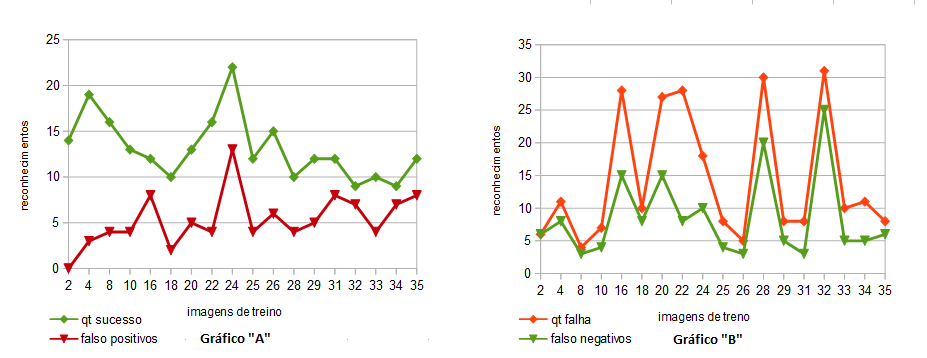
\includegraphics[width=1.1\textwidth]{grafab-fase12}
	\caption{\textbf{Gráfico "A"}: Reconhecimentos de sucesso (eixo Y) por quantidade de imagens usadas para o treino (eixo X). \textbf{Gráfico "B"}: Falhas no reconhecimentos (eixo Y) por quantidade de imagens usadas para o treino (eixo X). Referentes as fases de teste "1" e "2".}
	\fonte{Elaborado pelo autor.}
	\label{grafab-fase12}
\end{grafico}

\begin{grafico}[h]
	\centering
	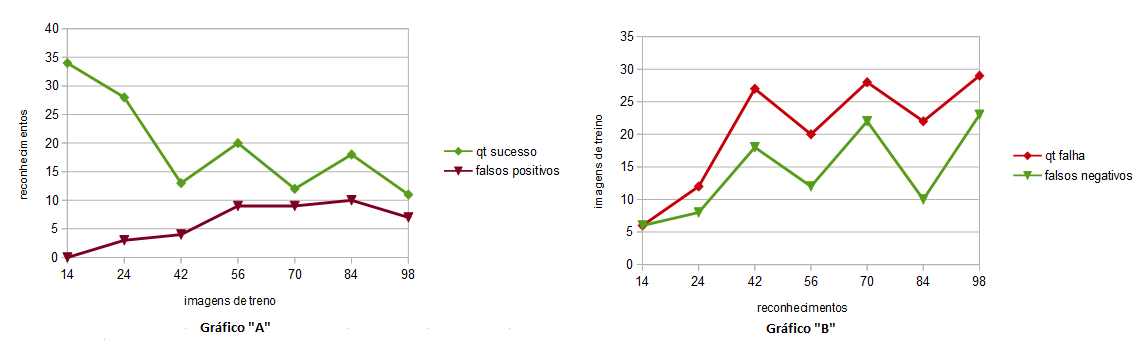
\includegraphics[width=1.1\textwidth]{grafab-fase3}
	\caption{\textbf{Gráfico "A"}: Reconhecimentos de sucesso (eixo Y) por quantidade de imagens usadas para o treino (eixo X). \textbf{Gráfico "B"}: Falhas no reconhecimentos (eixo Y) por quantidade de imagens usadas para o treino (eixo X). Referentes as fases de teste "3".}
	\fonte{Elaborado pelo autor.}
	\label{grafab-fase3}
\end{grafico}


Os \autoref{grafab-fase12} e \autoref{grafab-fase3} apresentam dois sub-gráficos "A"\ e "B": os gráficos "\textit{A}"\ são às contagens de reconhecimentos de sucesso (eixo \textit{Y}) a medida em que a quantidade de imagens de treino cresce (eixo \textit{X}), e os gráficos "\textit{B}", são as contagens de falhas de reconhecimento a medida em que as imagens de treinamento crescem. O \autoref{grafab-fase12} se refere aos resultados da fase "1"\ e "2", e o \autoref{grafab-fase3} é referente à fase "3". Foram divididos desta forma pelo fato de quem o espaço foi reiniciado no terceiro dia, como descreve a \autoref{ch:testresultfaz3}. 

Analisando-os, observa-se que nos dois gráficos "A", as linhas de quantidade de sucesso e falsos positivos tendem a se encontram enquanto que nos gráficos "B"\, o contrário acontece: as linhas de quantidade de falhas e de falsos negativos tendem a se afastar, apesar de não estar tão evidenciado \autoref{grafab-fase12} "B"\, podendo-se concluir que à medida em que o espaço multidimensional de \textit{eigenfaces} (\textit{eigenspace}) cresce, o método ACP apresenta distâncias falsas e verdadeiras similares, imprecisando seu veridito final.














%GRAFICOSSS PARA

%\begin{grafico}[h]
%	\centering
%	\fbox{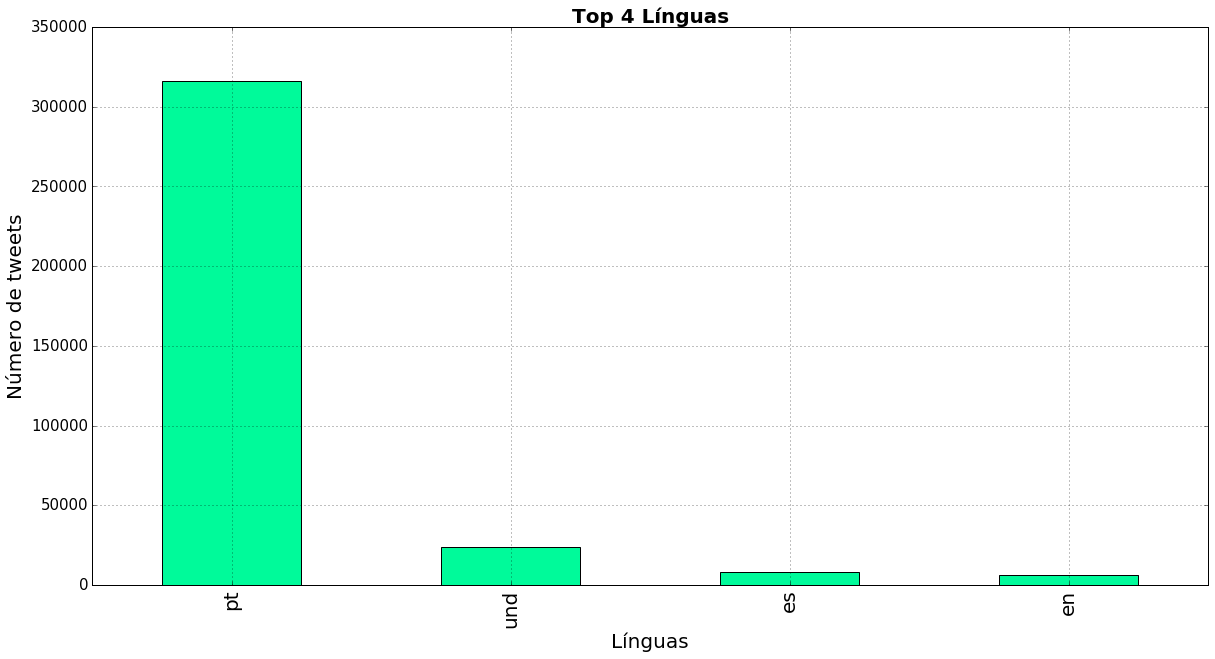
\includegraphics[width=1\textwidth]{linguas}}
%	\caption{Idiomas que mais realizaram \textit{tweets}}
%	\fonte{Elaborado pelo autor}
%	\label{lingua}
%\end{grafico}









